%%%%%%%%%%%%%%%%%%%%%%%%%%%%%%%%%%%%%%%%%
% Simple Sectioned Essay Template
% LaTeX Template
%
% This template has been downloaded from:
% http://www.latextemplates.com
%
% Note:
% The \lipsum[#] commands throughout this template generate dummy text
% to fill the template out. These commands should all be removed when 
% writing essay content.
%
%%%%%%%%%%%%%%%%%%%%%%%%%%%%%%%%%%%%%%%%%

%----------------------------------------------------------------------------------------
%	PACKAGES AND OTHER DOCUMENT CONFIGURATIONS
%----------------------------------------------------------------------------------------

\documentclass[12pt]{article} % Default font size is 12pt, it can be changed here

\usepackage{geometry} % Required to change the page size to A4
\geometry{a4paper} % Set the page size to be A4 as opposed to the default US Letter

\usepackage{graphicx} % Required for including pictures

\usepackage{float} % Allows putting an [H] in \begin{figure} to specify the exact location of the figure
\usepackage{wrapfig} % Allows in-line images such as the example fish picture

\usepackage{lipsum} % Used for inserting dummy 'Lorem ipsum' text into the template

\linespread{1.2} % Line spacing

%\setlength\parindent{0pt} % Uncomment to remove all indentation from paragraphs

\graphicspath{{Pictures/}} % Specifies the directory where pictures are stored

\begin{document}

%----------------------------------------------------------------------------------------
%	TITLE PAGE
%----------------------------------------------------------------------------------------

\begin{titlepage}

\newcommand{\HRule}{\rule{\linewidth}{0.5mm}} % Defines a new command for the horizontal lines, change thickness here

\center % Center everything on the page

\textsc{\LARGE University of Toronto}\\[1.5cm] % Name of your university/college
\textsc{\Large CSC321 Neural Network}\\[0.5cm] % Major heading such as course name
\textsc{\large Assignment 1}\\[0.5cm] % Minor heading such as course title

\HRule \\[0.4cm]
{ \huge \bfseries Face Recognition and Gender Classification with KNN}\\[0.4cm] % Title of your document
\HRule \\[1.5cm]

\begin{minipage}{0.4\textwidth}
\begin{flushleft} \large
\emph{Author:}\\
Tzu Yao \textsc{Chien} % Your name
\break
998758759 % Your name
\break
g2samuel
\end{flushleft}
\end{minipage}
~
\begin{minipage}{0.4\textwidth}
\begin{flushright} \large
\emph{Supervisor:} \\
Dr. Michael \textsc{Guerzhoy} % Supervisor's Name
\end{flushright}
\end{minipage}\\[4cm]

{\large \today}\\[3cm] % Date, change the \today to a set date if you want to be precise

%\includegraphics{Logo}\\[1cm] % Include a department/university logo - this will require the graphicx package

\vfill % Fill the rest of the page with whitespace

\end{titlepage}

%----------------------------------------------------------------------------------------
%	TABLE OF CONTENTS
%----------------------------------------------------------------------------------------

\tableofcontents % Include a table of contents

\newpage % Begins the essay on a new page instead of on the same page as the table of contents 

%----------------------------------------------------------------------------------------
%	INTRODUCTION
%----------------------------------------------------------------------------------------

\section{Part 1} % Major section




\begin{figure}[H] % Example image
  \centering 
  \begin{minipage}[b]{0.3\textwidth}
    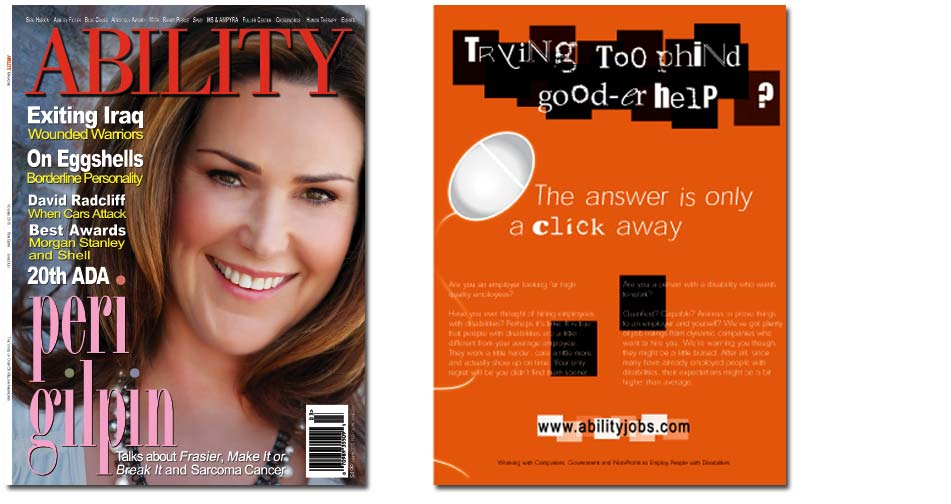
\includegraphics[width=\textwidth]{part1_1a}
    \caption{Uncropped Photo With Lots Noise.}
  \end{minipage}
  \begin{minipage}[b]{0.3\textwidth}
    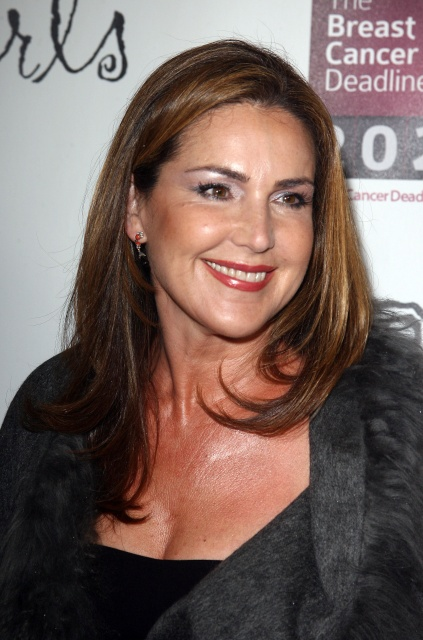
\includegraphics[width=\textwidth]{part1_1b}
    \caption{Uncropped Photo With Tilted Face.}
  \end{minipage}
  \begin{minipage}[b]{0.3\textwidth}
    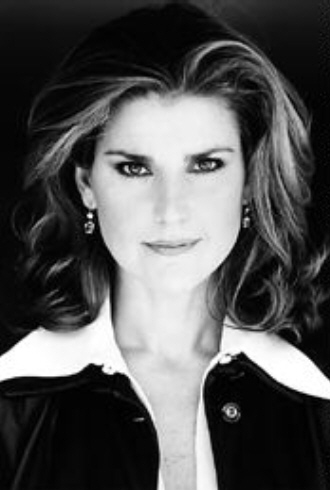
\includegraphics[width=\textwidth]{part1_1c}
    \caption{Uncropped Photo With Gray scale.}
  \end{minipage}
  \begin{minipage}[b]{0.3\textwidth}
    
\includegraphics[width=\textwidth]{part1_2a}
    \caption{Cropped and Gray Scale of the Above Figure}
  \end{minipage}
  \begin{minipage}[b]{0.3\textwidth}
    
\includegraphics[width=\textwidth]{part1_2b}
    \caption{Cropped and Gray Scale of the Above Figure}
  \end{minipage}
  \begin{minipage}[b]{0.3\textwidth}
    
\includegraphics[width=\textwidth]{part1_2c}
    \caption{Cropped and Gray Scale of the Above Figure}
  \end{minipage}
\end{figure}


After downloading the pictures from the address provided in  faces.txt file, I confirm the correctness of the photos using sha256 hash. This ensures the correctness of the photos matches the exact photos that’s been recorded in the database. These photos are different positions of different famous celebrities. The uncroppped pictures are all different. The difference includes colors, size, position of celebrities and all the noise in the pictures. First of all, the pictures comes in color and gray. The size of the photo also varies as well as the proportion of the celebrities faces in the pictures are also different. Moreover, the faces are also taken from variety of angles. As shown in the examples, there are a lot of different background and watermarks in the photo. Following the suggested cropped region, I was able to cropped the faces from the original photo and change it to gray scale then save it as 32x32 size. The cropped photo are mostly consistent where none of the faces are cut in half. However, due to the angle the photos are taken, the cropped images do not aligned with each other. Although I have resized the images to make all the cropped images similar, it is clear some photos are more blurry than the others. This is due to the fact that all the photos have different size of suggested cropping region. The photos are acceptable for further classification. 


%------------------------------------------------

\section{Part2} % Major section

I have downloaded and cropped 130 images for each of these actors 'Gerard Butler', 'Daniel Radcliffe', 'Michael Vartan', 'Lorraine Bracco', 'Peri Gilpin’, and 'Angie Harmon’. In other words, I just randomly picked first 100 photos of each actor as the training set, then use the next 10 faces as validation set, and the next 10 faces as test set. Step one, the goal is to have a dedicated training, validation, and test set to make sure our training for k does not overfit the validation set such that test set performance decrease. The test set should be independent of the training of validation percentage. The main drawback of this approach is that the variance for this approach might be high due to the fact that test set never changes. In other words, the more advance way to evaluate the performance of k should be using 10-fold cross validation where the test set, validation set, and training set changes. The result should be the average of 10 folds. 

%------------------------------------------------

\section{Part3} % Major section

\begin{figure}[H] % Example image
  \centering 
  \begin{minipage}[b]{0.7\textwidth}
    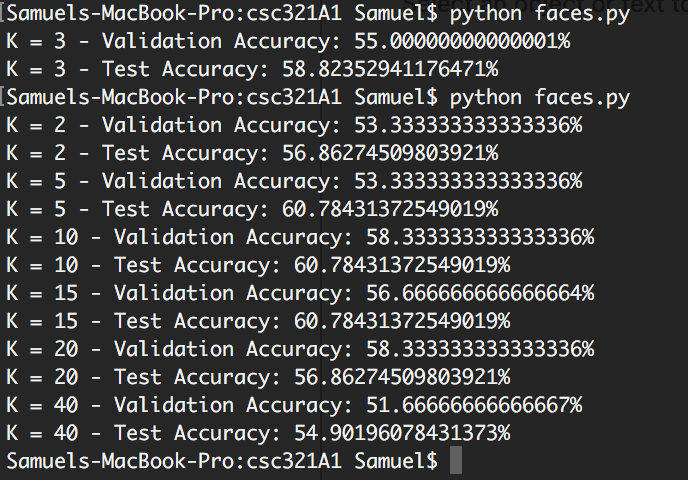
\includegraphics[width=\textwidth]{part3_2}
    \caption{KNN accuracy of Validation and Test Set}
  \end{minipage}
\end{figure}

In this section, I have tested a variety of k including 2, 5, 10, 15, 20, 40 and as shown in the performance output image, the accuracy of each validation and test set is recorded for each k value. 

\begin{figure}[H] % Example image
  \centering 
  \begin{minipage}[b]{0.7\textwidth}
    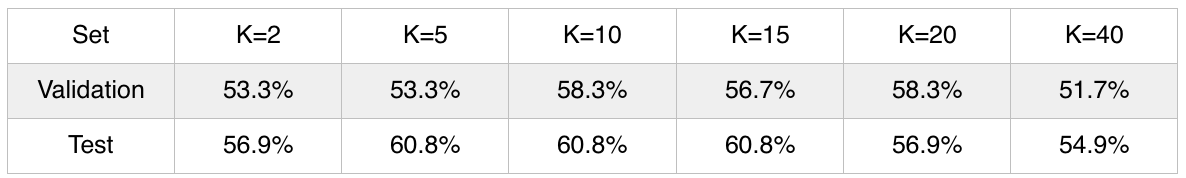
\includegraphics[width=\textwidth]{part3_0}
    \caption{Table: Accuracy of the Validation and Test Set}
  \end{minipage}
\end{figure}

From the table, we can clearly observe the trends where the accuracy of both set increases until the K=10 then it slowly decrease after the threshold. In other word, it is clear that K=10 is the best K. Keep in mind that this particular approach might have high variance since the validation and test set is constant. The best way to obtain the result with least variance is using 10-fold cross validation’s average result for each of the K value. 


\begin{figure}[H] % Example image
  \centering 
  \begin{minipage}[b]{0.7\textwidth}
    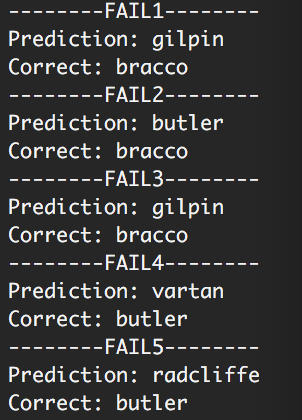
\includegraphics[width=\textwidth]{part3_1}
    \caption{Failure Cases of KNN}
  \end{minipage}
\end{figure}

Here I have also shown the first 5 failure case where KNN recognition is not correct as well as the the 5 Nearest Neighbors Face. As shown in the picture, I have observe that the KNN algorithm does not perform well when the pictures have similar color intensity. In addition, the tilted face or face expression can also influence the algorithm. 

\begin{figure}[H] % Example image
  \centering 
  \begin{minipage}[b]{0.2\textwidth}
    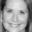
\includegraphics[width=\textwidth]{part3_3_1_correct_bracco}
    \caption{Target Image of Bracco}
  \end{minipage}
  \begin{minipage}[b]{0.1\textwidth}
    
\includegraphics[width=\textwidth]{part3_3_1_error1_bracco}
    \caption{1st Neighbor: Bracco}
  \end{minipage}
  \begin{minipage}[b]{0.1\textwidth}
    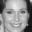
\includegraphics[width=\textwidth]{part3_3_1_error2_gilpin}
    \caption{2nd Neighbor: Gilpin}
  \end{minipage}
  \begin{minipage}[b]{0.1\textwidth}
    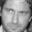
\includegraphics[width=\textwidth]{part3_3_1_error3_butler}
    \caption{3rd Neighbor: Butler}
  \end{minipage}
  \begin{minipage}[b]{0.1\textwidth}
    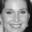
\includegraphics[width=\textwidth]{part3_3_1_error4_gilpin}
    \caption{4th Neighbor: Gilpin}
  \end{minipage}
  \begin{minipage}[b]{0.1\textwidth}
    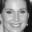
\includegraphics[width=\textwidth]{part3_3_1_error5_gilpin}
    \caption{5th Neighbor: Gilpin}
  \end{minipage}
\end{figure}

\begin{figure}[H] % Example image
  \centering 
  \begin{minipage}[b]{0.2\textwidth}
    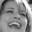
\includegraphics[width=\textwidth]{part3_3_2_correct_bracco}
    \caption{Target Image of Bracco}
  \end{minipage}
  \begin{minipage}[b]{0.1\textwidth}
    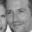
\includegraphics[width=\textwidth]{part3_3_2_error1_vartan}
    \caption{1st Neighbor: Vartan}
  \end{minipage}
  \begin{minipage}[b]{0.1\textwidth}
    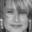
\includegraphics[width=\textwidth]{part3_3_2_error2_bracco}
    \caption{2nd Neighbor: Bracco}
  \end{minipage}
  \begin{minipage}[b]{0.1\textwidth}
    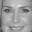
\includegraphics[width=\textwidth]{part3_3_2_error3_gilpin}
    \caption{3rd Neighbor: Gilpin}
  \end{minipage}
  \begin{minipage}[b]{0.1\textwidth}
    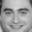
\includegraphics[width=\textwidth]{part3_3_2_error4_radcliffe}
    \caption{4th Neighbor: Radcli.}
  \end{minipage}
  \begin{minipage}[b]{0.1\textwidth}
    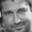
\includegraphics[width=\textwidth]{part3_3_2_error5_butler}
    \caption{5th Neighbor: Butler}
  \end{minipage}
\end{figure}


\begin{figure}[H] % Example image
  \centering 
  \begin{minipage}[b]{0.2\textwidth}
    
\includegraphics[width=\textwidth]{part3_3_3_correct_bracco}
    \caption{Target Image of Bracco}
  \end{minipage}
  \begin{minipage}[b]{0.1\textwidth}
    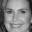
\includegraphics[width=\textwidth]{part3_3_3_error1_gilpin}
    \caption{1st Neighbor: Gilpin}
  \end{minipage}
  \begin{minipage}[b]{0.1\textwidth}
    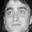
\includegraphics[width=\textwidth]{part3_3_3_error2_radcliffe}
    \caption{2nd Neighbor: Radcli.}
  \end{minipage}
  \begin{minipage}[b]{0.1\textwidth}
    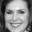
\includegraphics[width=\textwidth]{part3_3_3_error3_gilpin}
    \caption{3rd Neighbor: Gilpin}
  \end{minipage}
  \begin{minipage}[b]{0.1\textwidth}
    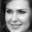
\includegraphics[width=\textwidth]{part3_3_3_error4_gilpin}
    \caption{4th Neighbor: Gilpin}
  \end{minipage}
  \begin{minipage}[b]{0.1\textwidth}
    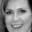
\includegraphics[width=\textwidth]{part3_3_3_error5_gilpin}
    \caption{5th Neighbor: Gilpin}
  \end{minipage}
\end{figure}

\begin{figure}[H] % Example image
  \centering 
  \begin{minipage}[b]{0.2\textwidth}
    
\includegraphics[width=\textwidth]{part3_3_4_correct_butler}
    \caption{Target Image of Butler}
  \end{minipage}
  \begin{minipage}[b]{0.1\textwidth}
    
\includegraphics[width=\textwidth]{part3_3_4_error1_butler}
    \caption{1st Neighbor: Butler}
  \end{minipage}
  \begin{minipage}[b]{0.1\textwidth}
    
\includegraphics[width=\textwidth]{part3_3_4_error2_butler}
    \caption{2nd Neighbor: Butler}
  \end{minipage}
  \begin{minipage}[b]{0.1\textwidth}
    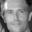
\includegraphics[width=\textwidth]{part3_3_4_error3_vartan}
    \caption{3rd Neighbor: Vartan}
  \end{minipage}
  \begin{minipage}[b]{0.1\textwidth}
    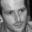
\includegraphics[width=\textwidth]{part3_3_4_error4_vartan}
    \caption{4th Neighbor: Vartan}
  \end{minipage}
  \begin{minipage}[b]{0.1\textwidth}
    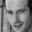
\includegraphics[width=\textwidth]{part3_3_4_error5_vartan}
    \caption{5th Neighbor: Vartan}
  \end{minipage}
\end{figure}

\begin{figure}[H] % Example image
  \centering 
  \begin{minipage}[b]{0.2\textwidth}
    
\includegraphics[width=\textwidth]{part3_3_5_correct_butler}
    \caption{Target Image of Butler}
  \end{minipage}
  \begin{minipage}[b]{0.1\textwidth}
    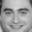
\includegraphics[width=\textwidth]{part3_3_5_error1_radcliffe}
    \caption{1st Neighbor: Radclif.}
  \end{minipage}
  \begin{minipage}[b]{0.1\textwidth}
    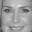
\includegraphics[width=\textwidth]{part3_3_5_error2_gilpin}
    \caption{2nd Neighbor: Gilpin}
  \end{minipage}
  \begin{minipage}[b]{0.1\textwidth}
    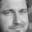
\includegraphics[width=\textwidth]{part3_3_5_error3_butler}
    \caption{3rd Neighbor: Butler}
  \end{minipage}
  \begin{minipage}[b]{0.1\textwidth}
    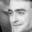
\includegraphics[width=\textwidth]{part3_3_5_error4_radcliffe}
    \caption{4th Neighbor: Radclif.}
  \end{minipage}
  \begin{minipage}[b]{0.1\textwidth}
    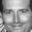
\includegraphics[width=\textwidth]{part3_3_5_error5_vartan}
    \caption{5th Neighbor: Vartan}
  \end{minipage}
\end{figure}

%------------------------------------------------

\section{Part4} % Major section

\begin{figure}[H] % Example image
  \centering 
  \begin{minipage}[b]{0.7\textwidth}
    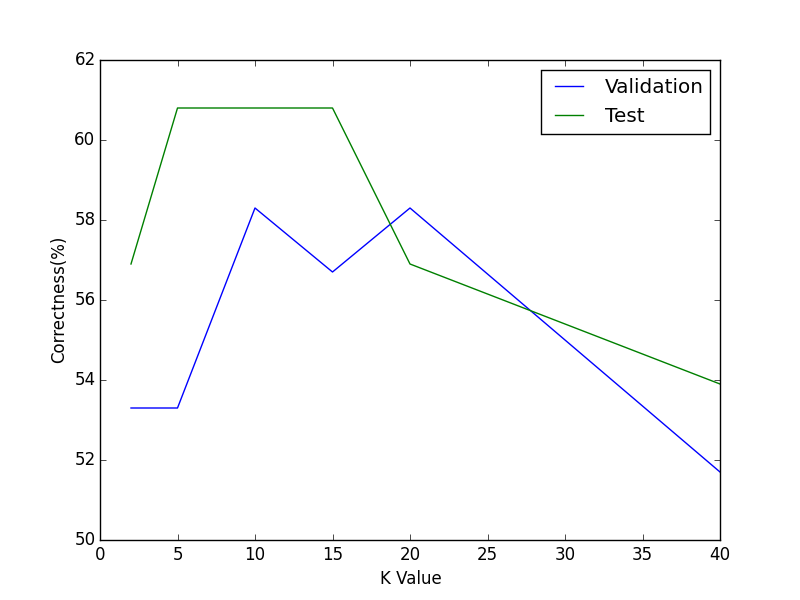
\includegraphics[width=\textwidth]{part4}
    \caption{Performance Chart of Test and Validation Set}
  \end{minipage}
\end{figure}

As shown in the chart, I have plotted the performance from part 3 and we can observe the trend easily. We can clearly observe the trends where the accuracy of both set increases until the K=10 then it slowly decrease after the threshold. The reason K=2’s accuracy is less than K=10 is because when K is too small, it can easily be influence by the outlier. On the other hand, when K is too big as K = 20, the result decrease significantly because the neighbor circle is too big and it doesn’t provide the fine grouping. 

%------------------------------------------------

\section{Part5} % Major section

\begin{figure}[H] % Example image
  \centering 
  \begin{minipage}[b]{0.7\textwidth}
    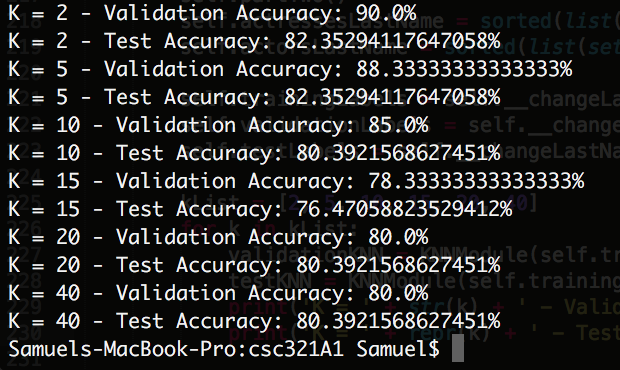
\includegraphics[width=\textwidth]{part5_1}
    \caption{Performance Output of Test and Validation Set}
  \end{minipage}
\end{figure}

In this section, I have tested a variety of k including 2, 5, 10, 15, 20, 40 and as shown in the performance output image, the accuracy of each validation and test set is recorded for each k value. 

\begin{figure}[H] % Example image
  \centering 
  \begin{minipage}[b]{0.7\textwidth}
    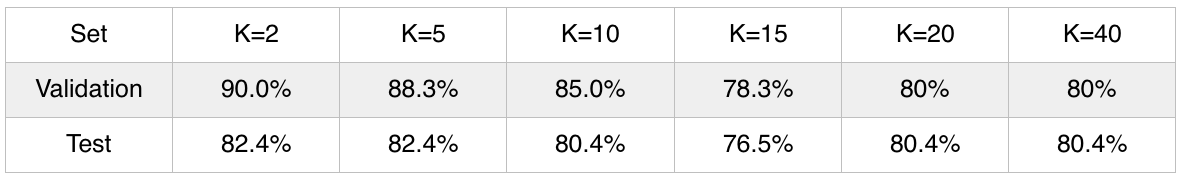
\includegraphics[width=\textwidth]{part5_3}
    \caption{Table: Accuracy of Test and Validation Set}
  \end{minipage}
\end{figure}

From the table, we can clearly observe the trends where the accuracy of both set started high at the K=2 then it slowly decrease after the threshold. The difference of part 5 and part 3 is that there is less classification and females generally look more alike, in other words, the data that’s closer together are likely in the same gender. Therefore, due to less classifications and nature of the gender images, it require less neighbor to determine the labels. In other word, it is clear that K=2 is the best K. Keep in mind that this particular approach might have high variance since the validation and test set is constant. The best way to obtain the result with least variance is using 10-fold cross validation’s average result for each of the K value. 

\begin{figure}[H] % Example image
  \centering 
  \begin{minipage}[b]{0.7\textwidth}
    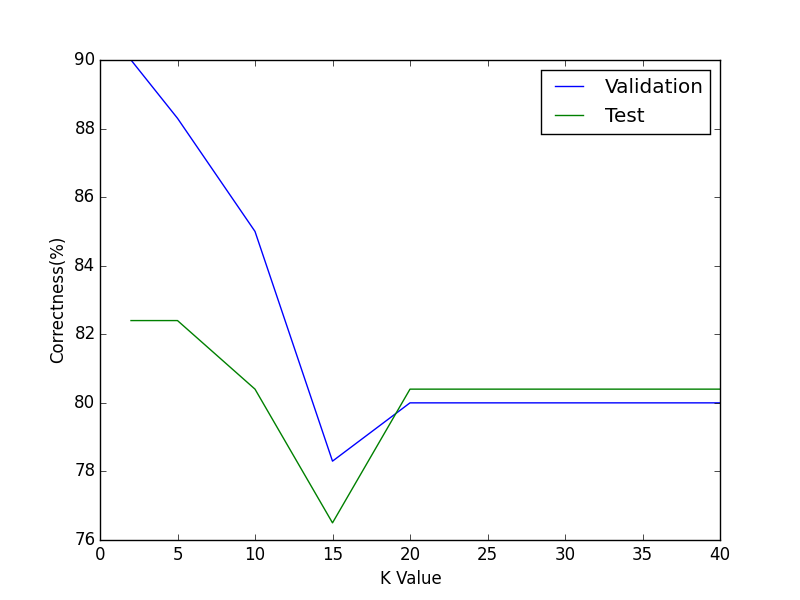
\includegraphics[width=\textwidth]{part5_2}
    \caption{Chart: Accuracy of Test and Validation Set}
  \end{minipage}
\end{figure}

As shown in the chart, I have plotted the performance from part 5 and we can observe the trend easily. We can clearly observe the trends where the accuracy of both set started high at K=2 then it slowly decrease after the threshold. The reason K=2’s accuracy is high is because there are only two labels and photo with same genders looks like each other. In other words, there is not many outliers which results high performance for small set of K. On the other hand, when K is too big as K = 20, the result decrease significantly because the neighbor circle is too big and it doesn’t provide the fine grouping.


%------------------------------------------------

\section{Part6} % Major section

\begin{figure}[H] % Example image
  \centering 
  \begin{minipage}[b]{0.7\textwidth}
    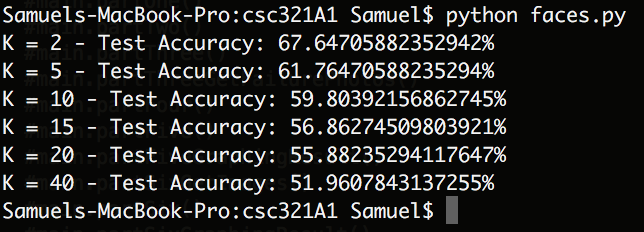
\includegraphics[width=\textwidth]{part6_1}
    \caption{Performance Output of Test and Validation Set}
  \end{minipage}
\end{figure}

In this section, I have tested a variety of k including 2, 5, 10, 15, 20, 40 and as shown in the performance output image, the accuracy of the people outside training set is recorded for each k value. (I take one of each person’s face in allFaces.txt)

\begin{figure}[H] % Example image
  \centering 
  \begin{minipage}[b]{0.7\textwidth}
    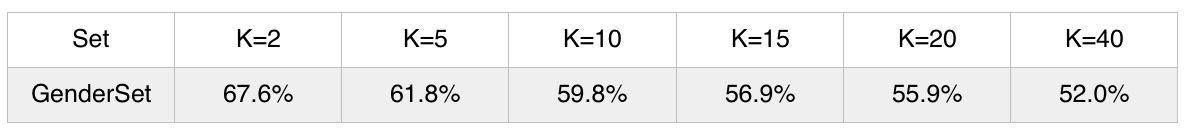
\includegraphics[width=\textwidth]{part6_3}
    \caption{Table: Accuracy of Test and Validation Set}
  \end{minipage}
\end{figure}

From the table, we can clearly observe the trends where the accuracy of both set started high at the K=2 then it slowly decrease after the threshold. The difference of part 5 and part 6 is that the test set are the people who’s not in the training set. In other words, it only works when there are two individual with same gender who looks alike. Therefore, due to the fact that all the celebrities have a pretty unique face features, the data is pretty scattered resulting better performance for smaller K. Through the test, it is clear that K=2 is the best K. Keep in mind that this particular approach might have high variance since the validation and test set is constant. The best way to obtain the result with least variance is using 10-fold cross validation’s average result for each of the K value. 

\begin{figure}[H] % Example image
  \centering 
  \begin{minipage}[b]{0.7\textwidth}
    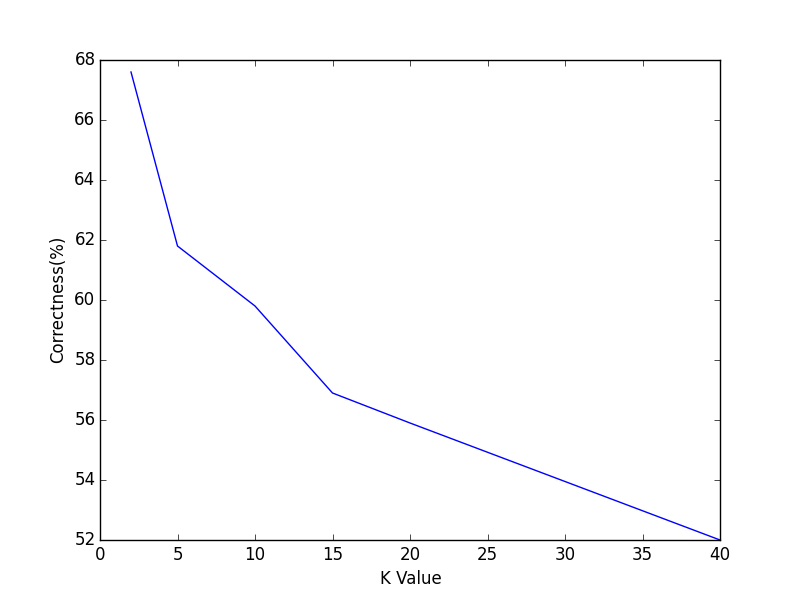
\includegraphics[width=\textwidth]{part6_2}
    \caption{Chart: Accuracy of Test and Validation Set}
  \end{minipage}
\end{figure}

As shown in the chart, I have plotted the performance from part 6 and we can observe the trend easily. We can clearly observe the trends where the accuracy of the set started high at K=2 then it slowly decrease after the threshold. The reason K=2’s accuracy is high is because there is little variance in euclid distances since most of the photo do not look like the distinct celebrities faces. In other words, the data is very clustered together which results high performance for small set of K. On the other hand, when K is too big as K = 20, the result decrease significantly because the neighbor circle is too big and it doesn’t provide the fine grouping.



\end{document}